\documentclass[a4paper,twocolumn,10pt]{article}
\usepackage{graphicx} % Required for inserting images

\title{Taller 3 y 4 Estructura de Datos}
\author{Camila Andrea Galindo Ruiz - 506222700 }
\date{10 Septiembre 2023}

\begin{document}

\maketitle

\section{Introduction}

La memorización es una técnica que implica almacenar y reutilizar resultados previamente calculados en lugar de volver a calcularlos cada vez que son necesarios.

En este artículo, nos adentraremos en el funcionamiento de un algoritmo diseñado para buscar. En el algoritmo desarrollado, se busca encontrar las palabras más comunes en un conjunto de documentos. Para lograrlo, el algoritmo utiliza una función recursiva. Esta función toma como entrada un índice que representa la posición actual en la lista de documentos. Aquí es donde entra en practica la memorización. Adicionalmente haremos la busqueda con otro algoritmo de una palabra específica dentro de un conjunto de frases o documentos. Se evidenciara cómo el algoritmo puede hacer que tu búsqueda de información sea mucho más eficiente.

Para el desarrollo de ambos algoritmos tenemos un documento base que cuenta con una cadena de frases. 

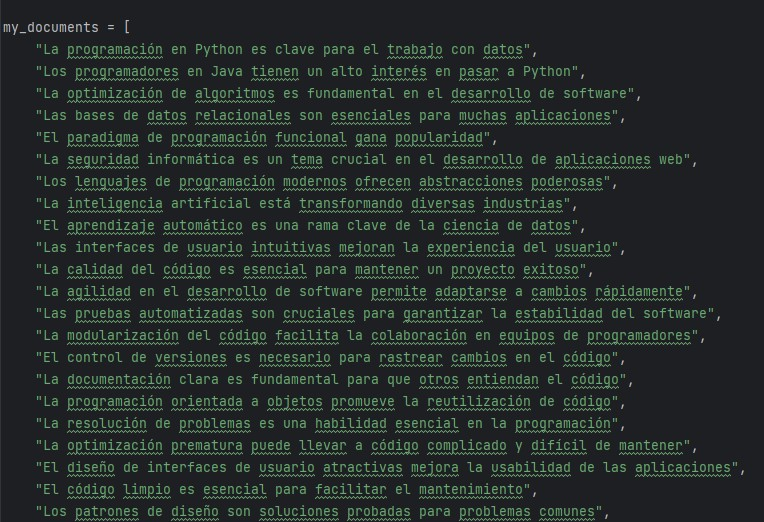
\includegraphics[width=0.8\linewidth]{imagenes/Programacion .jpg}

\section{Clasificacion de Palabras mas Repetidas }

En este codigo lo que se busca realizar es un top de las palabras que mas se repiten en la anterior cadena de frases. 

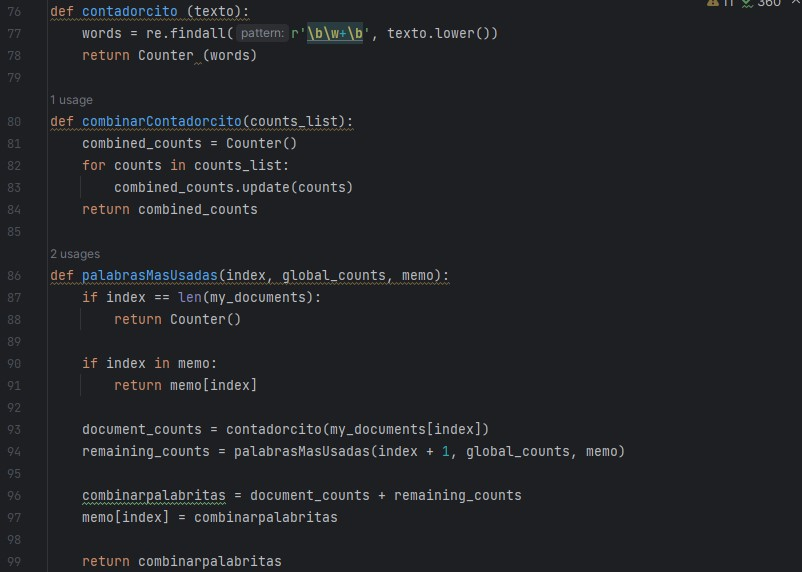
\includegraphics[width=0.8\linewidth]{imagenes/codigo 1.jpg}


1. Definir una función llamada `contadorcito(texto)` que toma un texto como entrada y realiza lo siguiente:
   - Convierte el texto a minúsculas esto ya que al comienzo de cada frase se encuentran los conectores en mayusculas y dentro de la oracion estos estan en minusculas y aunque sean la misma palabra se tomaria como diferentes. 
   - Utiliza la función `re.findall` para encontrar todas las palabras completas eliminando signos de puntuacion para que estos no sean tomados como palabras y no sean contados. Estas palabras se almacenan en la lista `palabritas`.
   - Devuelve un objeto `Counter` que cuenta la frecuencia de cada palabra en el texto.

2. Define una función llamada `combinarContadorcito` que toma una lista de objetos `Counter` como entrada y combina todas las cuentas en un solo objeto `Counter`. Esto se hace recorriendo la lista de recuentos y actualizando el contador combinado con cada recuento individual.

3. Define una función llamada $`palabrasMasUsadas$:

   La función realiza lo siguiente:
   Si $`index`$ es igual a la longitud de $`my_documents`$, significa que hemos procesado todos los documentos, por lo que devuelve un objeto $`Counter`$ vacío.
   Si $`index`$ ya está en el diccionario $`memo`$, devuelve el resultado previamente calculado en lugar de volver a calcularlo.
   Calcula el recuento de palabras en el documento actual utilizando la función $`contadorcito`$ y lo almacena en $`document counts`$.
   Luego, llama recursivamente a `palabrasMasUsadas` con `index + 1` para procesar el siguiente documento y almacena el resultado en $'remaining_counts`$.
   Combina los recuentos de palabras del documento actual y los documentos restantes en `combinarpalabritas`.
   Almacena `combinarpalabritas` en el diccionario `memo` para su uso futuro y lo devuelve como resultado.

4. Calcula el recuento global de palabras en todos los documentos llamando a `combinarContadorcito` con una lista de recuentos individuales para cada documento en $`my_documents`$. Esto se almacena en la variable $`contador_global`.$

5. Inicializa un diccionario `memo` para almacenar resultados intermedios.

6. Llama a la función $`palabrasMasUsadas`$con los argumentos iniciales $`0`$ para procesar el primer documento, $'contador global'$ para compartir el recuento global entre las llamadas recursivas y `memo` para almacenar resultados intermedios.

7. Calcula las 10 palabras más comunes en todos los documentos utilizando $`top_palabritas.most_common(10)`$.

8. Imprime las palabras más comunes junto con su frecuencia en orden descendente.

\section{Palabra Parametro }

Este código en Python realiza una búsqueda de una palabra específica en un conjunto de frases (documentos) y luego muestra las frases que contienen esa palabra. Paso a Paso:

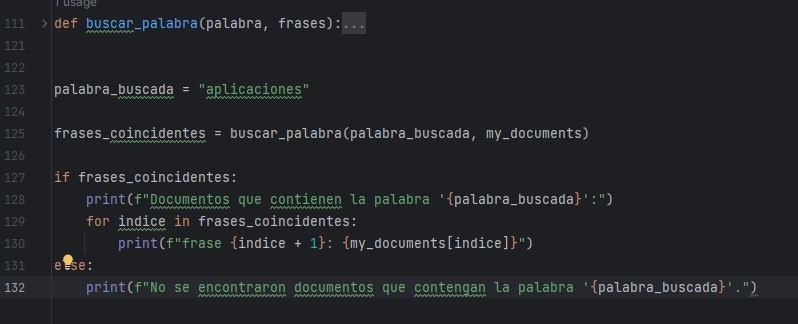
\includegraphics[width=0.8\linewidth]{imagenes/segundo codigo.jpg}


Se define una lista llamada $my_documents$ que contiene numerosas frases o documentos. Cada frase es un elemento de la lista.

Se define una función llamada $buscar_palabra$ que toma dos argumentos: palabra (la palabra que se quiere buscar) y frases (la lista de frases donde se realizará la búsqueda).

Se inicializa una lista vacía llamada $frases_coincidentes$ para almacenar los índices de las frases que contienen la palabra buscada.

A continuación, se inicia un bucle for que recorre cada elemento (frase) en la lista frases. Se utiliza enumerate para obtener tanto el índice i como la frase frases.

Dentro del bucle, la frase se convierte a minúsculas con frases.lower() y luego se divide en palabras individuales utilizando split(). Las palabras se almacenan en la lista palabras.

Se verifica si la palabra buscada (en minúsculas) está presente en la lista palabras. Si es así, se agrega el índice i de la frase a la lista $frases_coincidentes$.

Una vez que se ha recorrido todas las frases, la función retorna la lista $frases_coincidentes$ que contiene los índices de las frases que contienen la palabra buscada.

Fuera de la función, se especifica la palabra que se desea buscar en la variable $palabra_buscada$.

Se llama a la función $buscar_palabra$ con la palabra buscada y la lista de frases $my_documents$, y se almacena el resultado en la variable $frases_coincidentes$.

Luego, se verifica si hay frases coincidentes (si la lista $frases_coincidentes$ no está vacía). Si hay frases coincidentes, se imprime un mensaje que indica qué documentos contienen la palabra buscada y se muestra cada una de estas frases con su índice.

Si no se encontraron frases coincidentes, se imprime un mensaje que indica que no se encontraron documentos que contengan la palabra buscada.
\section{Complejidad Espacial y Temporal de los Algoritmos }

PRIMER ALGORITMO

La complejidad espacial y temporal del código se puede analizar de la siguiente manera:

1. Complejidad Espacial:
   - El espacio requerido para almacenar los documentos originales $(`my_documents`)$ es proporcional al número de documentos. En este caso, hay 100 documentos, por lo que esta parte del espacio es $O(100)$ o simplemente $O(n)$, donde "n" es el número de documentos.

   - El espacio requerido para almacenar el contador global $(`contador_global`)$ es proporcional al número total de palabras únicas en todos los documentos. Dado que no hay información sobre el número promedio de palabras por documento, esto se puede expresar como $O(w)$, donde "w" es el número total de palabras únicas en todos los documentos.

   - El espacio requerido para la variable `memo` es proporcional al número de documentos, ya que se almacena una entrada en la memoria por cada documento. Esto es $O(n)$ en este caso.

   - El espacio requerido para la variable $`top_palabritas`$ es proporcional al número de palabras únicas en todos los documentos, que es igual a la cantidad de palabras únicas en $`contador_global`$. Esto también es $O(w)$.

   Analizando la complejidad espacial total del código es $O(n + w)$, donde "n" es el número de documentos y "w" es el número total de palabras únicas en todos los documentos.

2. Complejidad Temporal:
    El cálculo del contador de palabras para cada documento se realiza en la función `contadorcito`. En general, si el tamaño promedio de los documentos es "m" y hay "n" documentos, el tiempo de ejecución de esta función sería $O(n * m)$.

   - En este caso, el número total de palabras únicas en todos los documentos es "w", por lo que esta función es $O(w)$.

   - La función `palabrasMasUsadas` es recursiva y procesa los documentos uno por uno. En el peor caso, se llamará a esta función una vez por cada documento, es decir, "n" veces. Dentro de la función, se realiza una operación de suma (combinación de contadores) que es lineal con respecto al número de palabras únicas en el documento actual. Por lo tanto, el tiempo de ejecución total de esta función es $O(n * w)$ en el peor caso.

   - Finalmente, la función $`most_common`$ se utiliza para encontrar las palabras más comunes en el contador global. Esto requiere ordenar el contador global, lo que tiene un tiempo de ejecución $O(w * log(w))$, donde "w" es el número de palabras únicas en todos los documentos.

   En resumen, la complejidad temporal total del código es $O(n * m + w * log(w))$, donde "n" es el número de documentos, "m" es el tamaño promedio de los documentos y "w" es el número total de palabras únicas en todos los documentos.

   SEGUNDO ALGORITMO
Complejidad Espacial:

1. $`my_documents`$: La variable almacena una lista de 100 documentos. Por lo tanto, el espacio requerido para almacenar `my_documents` es $O(n)$, donde "n" es 100.

2. $`frases_coincidentes`$: Es una lista que almacena los índices de las frases que contienen la palabra buscada. El espacio requerido para esta lista depende del número de frases que coinciden, pero en el peor caso, puede ser $O(n)$ si todas las frases coinciden.

En resumen, la complejidad espacial total del código es principalmente $O(n)$ debido a la lista $`my_documents`$ y a la lista $`frases_coincidentes`$.

Complejidad Temporal:

1. $`buscar_palabra`$: La función $`buscar_palabra`$ itera a través de cada frase en $`my_documents`$ para buscar si la palabra deseada está presente en esa frase. En el peor caso, esta función recorrerá todas las frases, por lo que su complejidad es O(n), donde "n" es el número de frases.

2. El bucle $`for`$ dentro de $`buscar_palabra`$ divide cada frase en palabras y verifica si la palabra deseada está presente. La división de una frase en palabras y la verificación de la coincidencia se realiza en tiempo lineal con respecto al número de palabras en cada frase. En el peor caso, cada frase tiene un número constante de palabras, por lo que esto es O(1).

3. La impresión de frases coincidentes también toma tiempo lineal con respecto al número de frases coincidentes, pero en el peor caso, esto puede ser O(n) si todas las frases coinciden.

En resumen, la complejidad temporal total del código es O(n), donde "n" es el número de frases en $`my_documents`$. El código no contiene bucles anidados ni estructuras de datos que escalen de manera significativa con el tamaño de entrada, lo que resulta en una complejidad lineal.
\section{Conclusion }

En resumen, el primer código recopila y procesa una lista de documentos, calcula la frecuencia de las palabras en cada documento y luego encuentra las palabras más comunes en todos los documentos.

En el segundo codigo la búsqueda de palabras clave en documentos es una tarea esencial en el análisis de texto y la minería de datos. Con este código de Python como ejemplo, los usuarios tienen una base sólida para desarrollar herramientas más avanzadas de procesamiento de texto que se adapten a sus necesidades específicas.


En general, los códigos tienen una complejidad temporal y espacial eficiente y no contiene bucles anidados ni estructuras de datos que escalen significativamente con el tamaño de entrada.

\section{Bibliografia  }

Lew, A., & Mauch, H. (2010). Dynamic programming: A computational tool. Springer.


Rivera, J. (2021, marzo 31). Introducción a la complejidad temporal de los algoritmos. freecodecamp.org. 
https://www.freecodecamp.org/espanol/news/introduccion-a-la-complejidad-temporal-de-los-algoritmos/



\end{document}
